% --- Preambolo coerente (se non già presente nel main) ---

\setlist{itemsep=2pt, topsep=4pt}
\newtheorem{theorem}{Theorem}[section]
\newtheorem{proposition}{Proposition}[section]
\newtheorem{corollary}{Corollary}[section]
\newtheorem*{remark}{Remark}

% =======================================================
\section{History and Why Mathematics Came In}
% =======================================================

\subsection{Definition of Cryptography}

The word \textbf{cryptography} originates from the Ancient Greek words \textit{κρυπτός} (\textit{kryptós}, “hidden, secret”) and \textit{γράφειν} (\textit{graphein}, “to write”). Therefore, cryptography literally means \textit{“the art of writing in secret”}.

\paragraph{Common misspellings.}
Crypthography, Criptography, Kryptography.

Cryptography has always been deeply connected with the need for secure communication. For thousands of years, rulers and generals relied on efficient communication to govern and lead armies, while fearing interception. This led to the invention of \textbf{codes} and \textbf{ciphers}: techniques for disguising a message so that only the intended recipient can understand it. Over the centuries, an arms race emerged between \textbf{code makers} and \textbf{code breakers}.

\begin{flushright}
\textit{(Source: Singh, \emph{The Code Book})}
\end{flushright}

\subsection{Terminology}

\begin{itemize}
  \item \textbf{Code:} replaces entire words with other words/symbols (e.g., “attack at dawn” $\rightarrow$ “JUPITER”).
  \item \textbf{Cipher:} replaces individual letters by a rule/pattern (e.g., a$\rightarrow$b, b$\rightarrow$c gives “attack at dawn” $\rightarrow$ “buubdl bu ebxo”).
  \item \textbf{Plaintext:} original message (lowercase).
  \item \textbf{Ciphertext:} encrypted message (uppercase).
\end{itemize}

In modern usage, \emph{decoding} and \emph{deciphering} are often used interchangeably. Today, virtually all practical systems are ciphers (codes are mostly obsolete).

\subsection{Classical Cryptography}

The earliest forms of cryptography are \textbf{classical ciphers}, e.g., the \emph{Caesar cipher}, where each letter is shifted by a fixed amount.

\begin{figure}[h!]
\centering
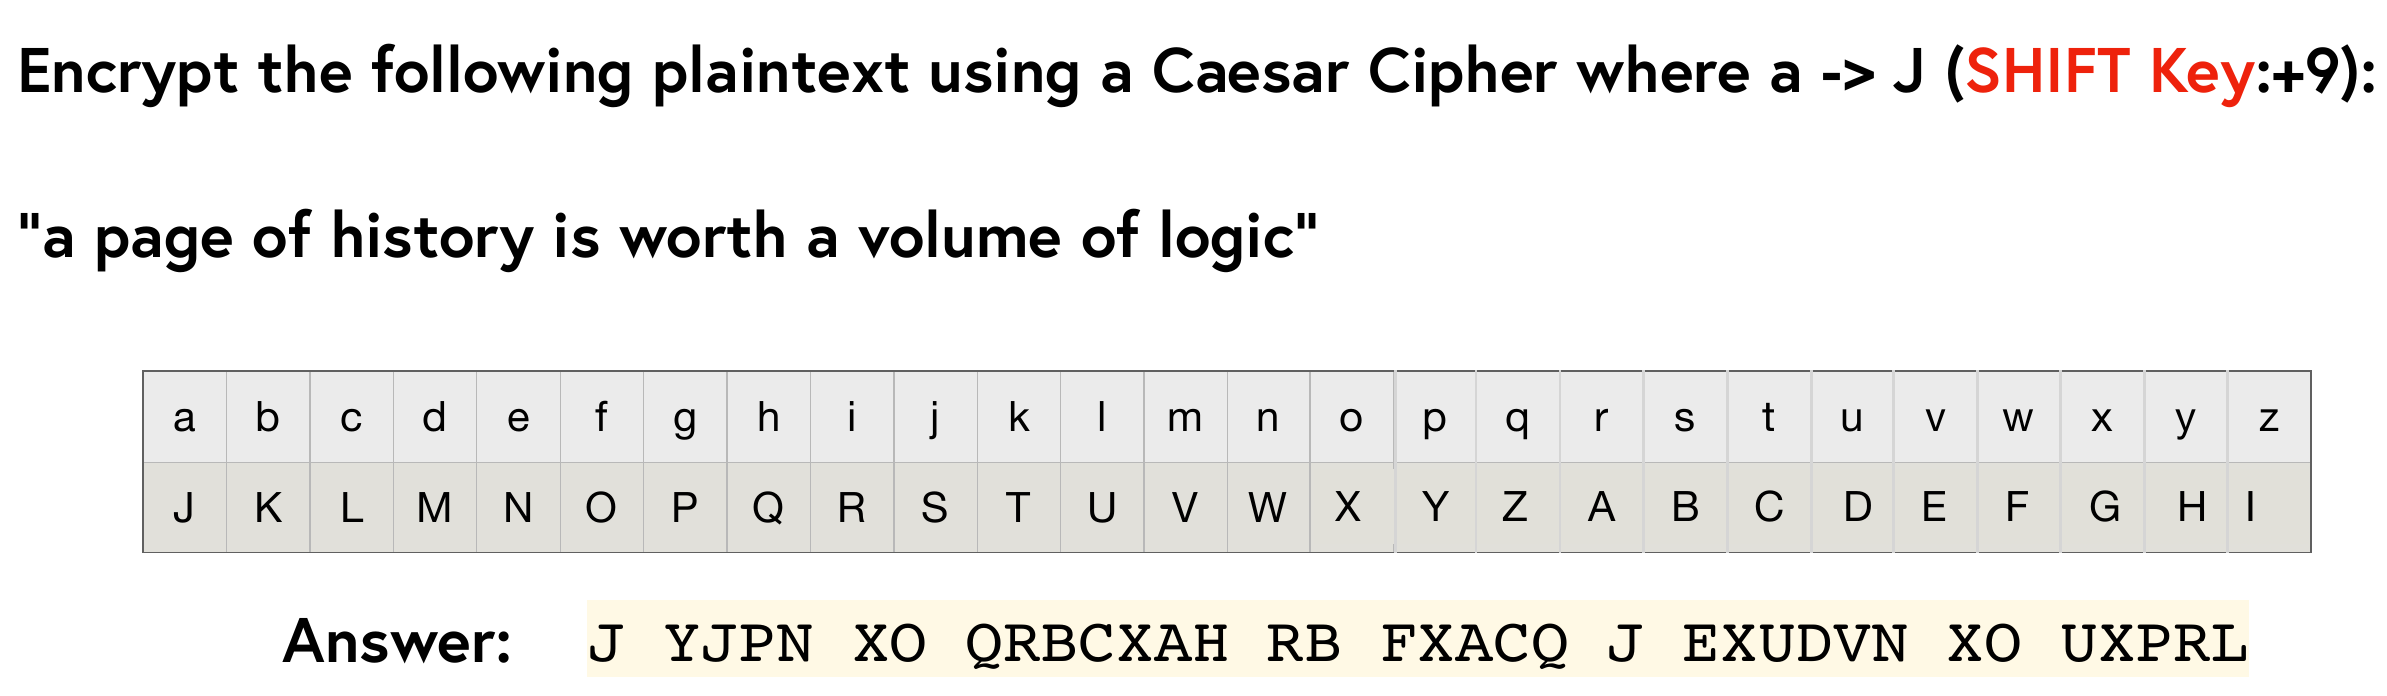
\includegraphics[width=0.7\textwidth]{Pictures/encrypt example.png}
\caption{Caesar cipher: each letter is shifted by a fixed number of positions.}
\label{fig:caesar_cipher}
\end{figure}

\subsection{Example of Decryption}

Decrypt the ciphertext \texttt{DVVKZECFSSPRKKVE} assuming a Caesar cipher.

\[
\text{Solution: } \texttt{meet in lobby at ten} \quad (\text{Key: } a \rightarrow R, \text{Shift } +17).
\]

This shows that a Caesar cipher has only \(\mathbf{26}\) possible keys (one per shift). A full monoalphabetic substitution, instead, admits \(26!\) keys:
\[
26! = 26 \times 25 \times \cdots \times 2 \times 1 \approx 4.03 \times 10^{26}.
\]

\subsection{Monoalphabetic Substitution Ciphers}

The \textbf{Caesar cipher} is a special case of \textbf{monoalphabetic substitution}. A general substitution can be any permutation of the \(26\) letters, hence:
\[
26! = 403{,}291{,}461{,}126{,}605{,}635{,}584{,}000{,}000.
\]
Even with \(10^{18}\) ops/s, a brute-force search would take on the order of years, showing that \emph{pure brute force} is impractical—yet these ciphers are still weak due to \emph{statistics}.

\subsection{The First Known Cryptanalyst: Al-Kindi}

In the 9th century, \textbf{Al-Kindi} wrote \emph{“A Manuscript on Deciphering Cryptographic Messages”}, introducing \textbf{frequency analysis}. Between 800–1200 AD, Arab scholars made major advances while Europe was in the Dark Ages; Al-Kindi laid foundations for cryptanalysis centuries before Europe.

\subsection{Frequency Analysis in English Texts}

Letters occur with different probabilities. In English, very common letters include:
\[
\text{e, t, a, o, i, n, s, h, r, d, l, u, m, w, c}.
\]
Digrams (pairs) like \texttt{th}, \texttt{he}, \texttt{in} are frequent:
\[
\texttt{th}\!:\,3.87\%,\quad \texttt{he}\!:\,3.69\%,\quad \texttt{in}\!:\,2.36\%.
\]

\subsection{Decrypting Using Frequency Analysis}

A monoalphabetic ciphertext can be attacked by matching ciphertext frequencies to language statistics (letters, digrams, trigrams), iteratively hypothesizing mappings to reconstruct plaintext. Computers automate these comparisons efficiently.

\subsection{Example: Decrypting a Long Ciphertext}

\begin{verbatim}
LIVITCSWPIYVEWHEVSRIQMXLEYVEOIEWHRXEXIPFEMVEWHKVSTYLXZIXLIKIIXPIJVSZEYPE...
\end{verbatim}

Frequency analysis reveals the plaintext progressively; for illustration:
\begin{quote}
\textit{“This course aims to introduce you to the principles and techniques of securing computers and networks, focusing on Internet security. You will learn both theoretical and practical aspects of cryptography, algorithms, and real-world security protocols.”}
\end{quote}

\subsection{Unit 2 — Modern Cryptography: Polyalphabetic Ciphers}

\subsubsection{Introduction to Polyalphabetic Ciphers}

The \textbf{Vigenère cipher} (Bellaso, 1550; later attributed to Vigenère) applies multiple shifting alphabets driven by a repeating keyword (e.g., key \(2,5,4,7\)). The same plaintext letter may encrypt to different ciphertext letters depending on position.

\subsubsection{Breaking the Vigenère Cipher}

\textbf{Kasiski} (19th c.) introduced a method to infer the \emph{key length} by detecting repeated sequences and factoring distances between repeats; common factors suggest candidate lengths (e.g., \(3\) and \(6\)).

\subsubsection{Frequency Analysis per Key Position}

Once the period is known, split the ciphertext into groups by position modulo the period; each group is a Caesar cipher and can be cracked by frequency analysis. Example outcome (period \(=3\)): shifts \((+2,\,0,\,+19)\).

\subsubsection{Revealing the Plaintext}

Decrypting with the recovered key yields readable plaintext. The method’s weakness: long reuse of a key exposes periodic patterns; one key per message is impractical.

\subsection{Historical Context: Codebreakers and the Evolution of Cryptography}

States have long employed \textbf{codebreakers}. Examples: \textbf{Mary, Queen of Scots} (1587) and the \textbf{Zimmermann Telegram} (1917) show strategic impact of cryptanalysis.

% =======================================================
\section{Cipher Machines}
% =======================================================

\subsection{The Rise of Cryptographic Machines (1920–1970)}

Radio/telegraph required secrecy over open channels; manual ciphers were replaced by \textbf{mechanical devices} enabling faster/stronger encryption.

\subsection{The Enigma Machine}

Invented by \textbf{Scherbius} (1918), later adopted by the German military. Enigma scrambles letters via electromechanical \textbf{rotors}; after each keypress, rotor stepping changes the mapping (like an odometer).

\subsection{The Rotors Mechanism}

Three rotors each implement a 26-letter permutation. Pressing a key advances rotor(s); thus the same plaintext letter encrypts differently at different times.

\subsection{The Reflector and the Plugboard}

A \textbf{reflector} returns the signal through the rotors (same setup for enc/dec). The \textbf{plugboard} swaps up to six letter pairs, adding confusion.
\[
\text{Path: Key} \to \text{Plugboard} \to \text{Rotors} \to \text{Reflector} \to \text{Rotors} \to \text{Plugboard} \to \text{Lampboard}.
\]

\subsection{Configuration Space of Enigma}

\begin{itemize}
  \item Rotor positions: \(26^3 = 17{,}576\).
  \item Rotor choices/order from 5: \(5 \cdot 4 \cdot 3 = 60\).
  \item Plugboard (6 pairs): \(\dfrac{26!}{14!\,2^6} \approx 1.0039\times 10^{11}\).
\end{itemize}
Total \(\approx 2\times 10^{17}\) configurations.

\subsection{Cracking Enigma — The Polish Breakthrough}

\textbf{Rejewski, Różycki, Zygalski} (1932) recovered rotor wirings using mathematics and intelligence. The doubled \emph{message key} created patterns exploitable via cycle structure; a large catalog enabled daily-key recovery in minutes (from 1934).

\subsection{Turing and the British Bombe}

German upgrades (1938) increased complexity. \textbf{Turing} designed the \textbf{Bombe}, exploiting stereotyped headers to test configurations quickly; crossword-style recruitment highlighted logic/language skills.

\subsection{The Lorenz Cipher and the Birth of the Computer}

High-level traffic used \textbf{Lorenz SZ40}. \textbf{Max Newman} led development of \textbf{Colossus} (1943), the first programmable digital computer, to attack Lorenz traffic. Post-war secrecy delayed public recognition.

% =======================================================
\section{Modern Cryptography (1970– )}
% =======================================================

\subsection{From Mechanical to Digital Cryptography}

Electronic computers enabled fast encryption/decryption but also brute-force attacks. Text is encoded in \textbf{ASCII}:
\[
\text{A}=01000001,\ \text{B}=01000010,\ \text{C}=01000011,\ \ldots
\]

\subsection{Lucifer and the Birth of DES}

IBM’s \textbf{Lucifer} (1971) evolved into \textbf{DES}, both \textbf{symmetric-key} ciphers combining substitution and transposition.

\subsection{The Problem of Private Keys}

Symmetric systems suffer from \textbf{key distribution}. Historical practice (e.g., Enigma daily keys) shows the logistical and security burden of sharing secrets safely.

\subsection{The Idea of Public Keys}

Goal:
\begin{quote}
\textit{How can Alice and Bob communicate securely over an eavesdropped channel without a pre-shared key?}
\end{quote}
The “double-lock” analogy motivates, but cryptographic ops need not commute—so a different idea is needed.

\subsection{Two Keys: One Private, One Public}

\textbf{Diffie \& Hellman} (1976) proposed separate \textbf{public} and \textbf{private} keys: encrypt with the recipient’s public key; decrypt with their private key.

\subsection{The Diffie–Hellman Key Exchange}

Public parameters: large prime \(p\), base \(g\). Alice picks \(a\), sends \(A=g^a\bmod p\); Bob picks \(b\), sends \(B=g^b\bmod p\). Shared secret:
\[
K=g^{ab}\bmod p=(g^a)^b\bmod p=(g^b)^a\bmod p.
\]
Security relies on the hardness of the discrete logarithm problem.

\subsection{The Digital Signature Problem}

DH provides secrecy but not authentication (vulnerable to MITM). Digital signatures address authenticity and integrity (concept by Diffie–Hellman; efficient schemes came later).

\subsection{The RSA Cryptosystem}

\textbf{Rivest–Shamir–Adleman} (1978) introduced \textbf{RSA} for public-key encryption and signatures, relying on the hardness of factoring \(N=pq\). (C. Cocks, GCHQ, discovered a similar idea in 1973—declassified in 1997.)

\subsection{Conclusion}

From Caesar to RSA, cryptography evolved with mathematics and computation. As computing advances, cryptography leans more on number theory and complex problems to stay ahead.

\begin{center}
\textit{“History and why Mathematics came in Cryptography.” — End of Lesson 1}
\end{center}
